\documentclass[12pt,oneside]{uhthesis}
\usepackage{subfigure}
\usepackage[ruled,lined,linesnumbered,titlenumbered,algochapter,spanish,onelanguage]{algorithm2e}
\usepackage{amsmath}
\usepackage{amssymb}
\usepackage{amsbsy}
\usepackage{caption,booktabs}
\captionsetup{ justification = centering }
%\usepackage{mathpazo}
\usepackage{float}
\setlength{\marginparwidth}{2cm}
\usepackage{todonotes}
\usepackage{listings}
\usepackage{xcolor}
\usepackage{multicol}
\usepackage{graphicx}
\floatstyle{plaintop}

\restylefloat{table}
\usepackage{biblatex}
\addbibresource{Bibliography.bib}
% \setlength{\parskip}{\baselineskip}%
\renewcommand{\tablename}{Tabla}
\renewcommand{\listalgorithmcfname}{Índice de Algoritmos}
%\dontprintsemicolon
\SetAlgoNoEnd

\definecolor{codegreen}{rgb}{0,0.6,0}
\definecolor{codegray}{rgb}{0.5,0.5,0.5}
\definecolor{codepurple}{rgb}{0.58,0,0.82}
\definecolor{backcolour}{rgb}{0.95,0.95,0.92}

\lstdefinestyle{mystyle}{
    backgroundcolor=\color{backcolour},   
    commentstyle=\color{codegreen},
    keywordstyle=\color{purple},
    numberstyle=\tiny\color{codegray},
    stringstyle=\color{codepurple},
    basicstyle=\ttfamily\footnotesize,
    breakatwhitespace=false,         
    breaklines=true,                 
    captionpos=b,                    
    keepspaces=true,                 
    numbers=left,                    
    numbersep=5pt,                  
    showspaces=false,                
    showstringspaces=false,
    showtabs=false,                  
    tabsize=4
}

\lstset{style=mystyle}

\title{Generación Automática de Reportes a partir de Consultas en Lenguaje Natural sobre Bases de Conocimiento.}
\author{\\\vspace{0.25cm}David Cabrera García}
\advisor{\\\vspace{0.25cm}DrC. Alejandro Piad Morffis}
\degree{Licenciado en Ciencia de la Computación}
\faculty{Facultad de Matemática y Computación}
\github{\href{https://github.com/DavidCabrera9943/automate\_report\_generation}{https://github.com/DavidCabrera9943/automate\_report\_generation}}
\logo{Graphics/uhlogo}
\makenomenclature

\renewcommand{\vec}[1]{\boldsymbol{#1}}
\newcommand{\diff}[1]{\ensuremath{\mathrm{d}#1}}
\newcommand{\me}[1]{\mathrm{e}^{#1}}
\newcommand{\pf}{\mathfrak{p}}
\newcommand{\qf}{\mathfrak{q}}
%\newcommand{\kf}{\mathfrak{k}}
\newcommand{\kt}{\mathtt{k}}
\newcommand{\mf}{\mathfrak{m}}
\newcommand{\hf}{\mathfrak{h}}
\newcommand{\fac}{\mathrm{fac}}
\newcommand{\maxx}[1]{\max\left\{ #1 \right\} }
\newcommand{\minn}[1]{\min\left\{ #1 \right\} }
\newcommand{\lldpcf}{1.25}
\newcommand{\nnorm}[1]{\left\lvert #1 \right\rvert }
\renewcommand{\lstlistingname}{Ejemplo de código}
\renewcommand{\lstlistlistingname}{Ejemplos de código}

\begin{document}

\frontmatter
\maketitle

\begin{dedication}
    A mis padres.
\end{dedication}
\begin{acknowledgements}
  Quiero agradecer a todas las personas que me acompañaron en este camino, haciendo posible este logro, en especial, a mi familia. A mis padres, gracias por creer en mí, por su paciencia infinita, sus sabios consejos y por los innumerables sacrificios que hicieron para que pudiera llegar hasta aquí. A mi hermano gracias por estar siempre presente, por tu comprensión y por compartir conmigo este camino, tu aliento en los momentos difíciles y tu alegría en los logros fue una constante inspiración para seguir adelante. Finalmente, a todos aquellos que, de una u otra manera, aportaron su granito de arena para la realización de esta tesis. 
\end{acknowledgements}
\include{FrontMatter/SupervisorOpinion}
\begin{resumen}
	Esta tesis explora la automatización de la generación de reportes utilizando Modelos de Lenguaje Grandes (LLMs) y bases de conocimiento estructuradas. Abordando las ineficiencias de la creación manual de reportes. La solución propuesta integra las capacidades generativas de los LLMs con la recuperación de información desde datos estructurados. El sistema implementado utiliza LLMs de código abierto y técnicas de prompt engineering, incluyendo la decodificación Skeleton-of-Thought, para generar reportes coherentes e informativos a partir de consultas en lenguaje natural con una arquitectura modular que facilita la adaptabilidad y extensibilidad
\end{resumen}

\begin{abstract}
	This thesis explores the automation of report generation using Large Language Models (LLMs) and structured knowledge bases. Addressing the inefficiencies of manual report creation, the proposed solution integrates the generative capabilities of LLMs with information retrieval from structured data. The implemented system leverages open-source LLMs and prompt engineering techniques, including Skeleton-of-Thought decoding, to generate coherent and informative reports from natural language queries with a modular architecture that facilitates adaptability and extensibility.
\end{abstract}
\tableofcontents
\listoffigures
% \listoftables
% \listofalgorithms
%\lstlistoflistings

\mainmatter

\chapter*{Introducción}\label{chapter:introduction}
\addcontentsline{toc}{chapter}{Introducción}

Desde la década de 1950, se ha intentado dotar a las computadoras con capacidades de razonamiento y entendimiento del lenguaje humano. La creación de una máquina capaz de simular a un humano siempre ha sido uno de los principales objetivos de las ciencias de la computación. Para esto, se ha investigado en áreas como la lógica simbólica, la lingüística computacional y el aprendizaje automático, buscando emular la complejidad del pensamiento y la comunicación humana. Un paso crucial en este camino es el Procesamiento del Lenguaje Natural (PLN), cuyo objetivo es capacitar a las máquinas para entender, interpretar y generar lenguaje humano de manera efectiva. Los primeros acercamientos en este campo fueron de naturaleza simbólica, con sistemas como ELIZA y SHRDLU en la década de 1960, que utilizaban reglas predefinidas para procesar y responder a entradas de texto. En la década de 1980, el enfoque cambió hacia métodos estadísticos, impulsados por el aumento del poder computacional y la disponibilidad de grandes corpus de texto. Modelos como los de alineación de IBM para la traducción automática marcaron un hito en esta época. Sin embargo, fue la llegada de las redes neuronales profundas y la publicación del artículo 'Attention is All You Need' en 2017 lo que marcó un antes y un después en el PLN. La introducción de los 'Transformers' y la atención como mecanismo clave permitieron avances sin precedentes en tareas como la traducción automática, el resumen de texto y la generación de lenguaje, llevando al PLN a un reconocimiento a nivel mundial no solo dentro de las ciencias de la computación, sino tambien en otras disciplinas.

Este giro hacia las redes neuronales profundas, y en particular a los modelos de lenguaje grandes (LLMs), ha tenido un impacto significativo en el sector empresarial. La capacidad de automatizar tareas relacionadas con el lenguaje ha abierto un abanico de posibilidades para la optimización de procesos. Las empresas han comenzado a utilizar el PLN para la extracción de información de grandes volúmenes de documentos, el análisis de sentimientos en redes sociales para entender la percepción de la marca, y la creación de chatbots más sofisticados para la atención al cliente. La automatización de estas tareas no solo aumenta la eficiencia, sino que también permite a las empresas obtener información valiosa de datos que antes eran inaccesibles, impulsando la toma de decisiones basada en datos y la innovación en diversos sectores.

La automatización de tareas se ha convertido en una fuerza transformadora en el panorama actual, impulsada por la creciente necesidad de eficiencia y optimización en diversos sectores, principalmente los negocios y finanzas. En este contexto, la generación automática de reportes a partir de una consulta en lenguaje natural surge como un campo de investigación y desarrollo de gran relevancia, principalmente en entornos donde la información precisa y oportuna es esencial para la toma de decisiones estratégicas y operativas. Tradicionalmente, la elaboración de reportes ha sido un proceso manual, exigiendo un considerable consumo de tiempo, recursos humanos y económicos. La necesidad de contar con personal altamente preparado asi como una base de datos lo sificientemente precisa ha hecho que las empresas inviertan gran cantidad de dinero en personal y recursos que permitan elaborar reportes cada vez mas complejos debido a la creciente cantidad de datos que son recolectados actualmente. Sin embargo, los notables avances en el campo del Procesamiento del Lenguaje Natural (PLN) y la Inteligencia Artificial (IA), con la aparición de los Modelos de Lenguaje Generativos (LLMs), abren nuevas perspectivas para la automatización de esta tarea, prometiendo una mayor eficiencia, escalabilidad y reducción de costos.
Basándonos en casos de uso empresarial comunes, como informes de análisis financiero, respuestas a solicitudes de propuestas y documentación técnica, se estima que la generación de informes puede ahorrar entre 10 y 15 horas por informe al automatizar el trabajo inicial de redacción y formato. Para los equipos que producen docenas de informes mensuales, esto puede traducirse en miles de horas anuales que se pueden redirigir a análisis de alto valor y trabajo estratégico.

Los Modelos de Lenguaje Generativos (LLMs), como la familia GPT-*, LaMDA, Gemini y otros, representan una revolución en el campo del PLN.  Estos modelos, construidos con arquitecturas de redes neuronales profundas basadas en *transformers*, han demostrado una capacidad notable para generar texto de alta calidad, imitando el estilo y la estructura del lenguaje humano. Su entrenamiento se basa en el aprendizaje de relaciones estadísticas a partir de vastas cantidades de texto lo que les permite generar texto coherente, relevante y adaptable a diferentes contextos y propósitos. Los LLMs han encontrado aplicaciones en diversas áreas, desde la traducción automática y la generación de contenido creativo hasta la creación de código y la interacción con usuarios en *chatbots*. Siendo estos dos ultimos puntos vitales para el desarrollo del trabajo actual, dotar a un LLM de todos los datos como contexto para que este genere información y permita dar una respuesta coherente a un usuario, no es factible con la capacidad de cómputo y los modelos actuales, es ahí donde entra en juego su capacidad de generación de código, el cual, le permita acceder a los datos necesarios para la solicitud del usuario en cuestión. No obstante, a pesar de sus impresionantes capacidades, los LLMs presentan ciertas limitaciones, especialmente cuando se trata de generar reportes extensos, complejos y con un alto grado de especificidad.

Una de las principales deficiencias de los LLMs radica en su dificultad para mantener la coherencia y la precisión a medida que aumenta la extensión del texto generado. En reportes que requieren una estructura narrativa compleja y una cohesión rigurosa, los LLMs pueden incurrir en repeticiones, divagaciones o incluso introducir información errónea o inconsistente. Esta limitación se agudiza en dominios específicos, donde el conocimiento especializado, la terminología precisa y el rigor científico son requisitos fundamentales. Los LLMs, entrenados en corpus de texto de propósito general, pueden carecer de la comprensión profunda y el contexto específico necesarios para producir reportes que cumplan con los estándares de calidad y precisión exigidos en áreas como la medicina, el derecho, la ingeniería o las finanzas.

Además, los LLMs pueden mostrar sesgos y prejuicios presentes en los datos de entrenamiento, lo que puede llevar a la generación de contenido no equitativo o incluso discriminatorio. Estos sesgos pueden manifestarse en la representación injusta de grupos demográficos o en la amplificación de estereotipos sociales, lo que plantea serias preocupaciones éticas y de responsabilidad en la aplicación de estas tecnologías. Para la generación de reportes, esto puede traducirse en conclusiones tendenciosas o en la omisión de información relevante.

Para reducir estos efectos, actualmente se está trabajando en distintas estrategias que permitan generar informes cada vez más largos que mantengan una cierta concordancia y reduzcan la divagación o las repeticiones. Una estrategia prometedora para esto es la decodificación con esqueleto de pensamiento o Skeleton-of-Thought Decoding, que se centra principalmente en dividir la generación del informe en dos etapas: primero, la creación de un esqueleto o esquema de alto nivel del contenido del informe, y segundo, la expansión detallada de cada punto del esqueleto. Lo que permite un mejor control sobre la estructura y el contenido del reporte, y además la paralelización del segundo paso, lo que influye en resultados más rápidos generalmente. Esta estrategia busca emular el proceso humano de organizar ideas antes de desarrollarlas completamente, lo cual resulta en un reporte mejor estructurado y con menos repeticiones.

Adicionalmente, en la búsqueda de sistemas robustos para la generación de reportes, se ha identificado la necesidad de abordar el problema de manera más integral, utilizando una serie de bloques de construcción fundamentales que pueden mejorar la calidad y eficiencia del proceso. Estos bloques, que se centran en controlar la forma y el contenido del reporte, incluyen: la definición de salida estructurada, la cual establece claramente el formato y los tipos de contenido que debe incluir el reporte, usando esquemas definidos para diferentes tipos de contenido; el procesamiento avanzado de documentos, que permite analizar la información de distintas fuentes de datos (como PDFs, presentaciones, hojas de cálculo, etc.) y entender su estructura (tablas, imágenes, gráficos); la integración de una base de conocimiento, que actúa como el motor del sistema, almacenando, recuperando y gestionando información multimodal, manteniendo metadatos relevantes como la frescura y pertinencia de los datos; una arquitectura de flujo de trabajo multiagente, que delega tareas específicas a diferentes agentes, como la recuperación de información, la redacción y la edición, replicando el flujo de trabajo de equipos de redacción humanos y resultando en un contenido de mejor calidad; y un sistema de procesamiento de plantillas, el cual permite usar formatos existentes y mapear la información a las diferentes secciones, cumpliendo con los estándares organizacionales. Estos componentes funcionan juntos en un pipeline donde, tras una solicitud de reporte, el sistema analiza el formato requerido, recupera información, genera contenido estructurado y revisa la salida antes de la entrega final, asegurando una alta consistencia y automatización, con una necesaria revisión humana de documentos críticos.

Para superar estas limitaciones, este trabajo propone una solución computacional que combina las capacidades generativas de los LLMs con el acceso a una base de conocimiento estructurado. La hipótesis principal es que al proporcionar a los LLMs una fuente de información precisa, verificada y específica del dominio, se puede mejorar significativamente la calidad, precisión y coherencia de los reportes generados. Esta integración permite a los LLMs basar sus respuestas en datos concretos y actualizados, evitando la generación de información falsa o irrelevante.  Adicionalmente, la estructuración de la base de conocimiento facilita la extracción automática de la información relevante para el reporte, asegurando que el contenido generado sea completo y esté ajustado a las necesidades del usuario.

La solución que se propone se apoya en dos estrategias fundamentales: la extracción de contenido relevante a partir de una consulta en lenguaje natural y el uso de técnicas de *prompt engineering* para guiar la generación del reporte. La primera estrategia se enfoca en desarrollar un mecanismo que permita traducir las consultas del usuario, expresadas en lenguaje natural, en una serie de consultas estructuradas a la base de conocimiento. Este proceso asegurará que la información extraída sea la precisa y pertinente para la generación del reporte, adaptándola a las necesidades específicas del usuario. La segunda estrategia, el *prompt engineering*, se centra en el diseño de instrucciones precisas y contextualizadas para el LLM, de modo que pueda integrar la información extraída de la base de conocimiento de forma coherente y estructurada. El *prompt* servirá como una guía para el LLM, proporcionándole el contexto y la estructura, necesarios para generar un reporte que cumpla con los requisitos de estilo, formato y contenido.


\chapter{Estado del Arte}\label{chapter:state-of-the-art}

La generación automática de reportes, impulsada por la necesidad de procesar y comunicar grandes volúmenes de información de manera eficiente y comprensible, es un área de investigación en constante evolución. Este capítulo presenta una revisión de la literatura relevante, enfocándose en la generación de código para preprocesamiento de datos y la construcción de reportes a partir de bases de conocimiento estructuradas, utilizando modelos de lenguaje grandes (LLMs) y técnicas de recuperación de información.

\section{Generación de Código y Consultas}

La generación automática de fórmulas y consultas, ya sea SQL o pandas, es de vital importancia para el análisis de datos. FLAME \cite{joshi2024flame} es un modelo basado en T5(Text-to-Text Transfer Transformer)\cite{raffel2020exploring} entrenado específicamente para generar fórmulas de Excel. Aunque este es efectivo en tareas como la reparación y completación de fórmulas, su aplicación se limita al entorno de Excel y a fórmulas predefinidas. Mientras que LLMs como GPT-4 y Claude-2 han demostrado una gran capacidad en tareas de conversión de texto-SQL, su evaluación se ha centrado en bases de datos pequeñas, a diferencia de las grandes bases de datos del mundo real.

BIRD \cite{li2024can} proporciona un benchmark más realista para la evaluación de la conversión de texto a SQL en bases de datos grandes y con mayor variedad de datos lo cual lo acerca más a un escenario práctico. También presenta tres desafíos: el manejo de bases de datos grandes y sucias, la maximización de la efectividad de la ejecución de SQL y la evaluación de fuentes de información externas. Si bien BIRD hizo posible que los usuarios accedieran y modificaran bases de datos sin necesidad de conocimientos de programación, este enfoque se limita al uso de SQL; Como el preprocesamiento de datos generalmente se realiza con Python, es bastante engorroso escribir procedimientos complejos en SQL.

\section{LLMs con Recuperación de Información}

La integración de LLMs con técnicas de recuperación de información, como en la Generación Aumentada por Recuperación (RAG) \cite{lewis2020retrieval}, ha revolucionado la generación de texto, mejorando significativamente la precisión, especificidad y diversidad del lenguaje generado. RAG combina la potencia generativa de los LLMs con la capacidad de acceder y manipular información externa, superando las limitaciones inherentes de los modelos paramétricos secuencia-a-secuencia y las arquitecturas de recuperación-y-extracción específicas de tareas.

El desarrollo de los LLMs ha provocado un cambio de paradigma en como los humanos adquirimos la información, cambiando de recibir la información a través de las búsquedas, a generar información con dichos resultados. Como resultado de esto, los sistemas de recuperación de información ahora trabajan para los LLMs en vez de para los humanos. Trabajos como Self-Retrieval \cite{tang2024self} replantean la arquitectura de la recuperación de información, internalizando documentos dentro del LLM y redefiniendo la búsqueda como un proceso de generación y autoevaluación dentro del propio modelo.

El auge de las bases de datos vectoriales, como Qdrant \cite{qdrant} y Pinecone \cite{pinecone}, ha impulsado la adopción de pipelines LLM y RAG. Estas bases de datos, que almacenan vectores embebidos y datos, permiten búsquedas rápidas y precisas de los vecinos más cercanos a un vector de consulta mediante algoritmos de búsqueda aproximada de vecinos más cercanos, facilitando el aprendizaje de los LLMs a partir de grandes conjuntos de datos. Esta sinergia entre recuperación de información y generación de lenguaje ha difuminado la línea que las separa, transformando la manera en que los humanos adquieren información, pasando de la búsqueda tradicional a la generación de información a través de LLMs. En consecuencia, los sistemas de recuperación de información ahora sirven de apoyo tanto a humanos como a LLMs.

\section{Preprocesamiento de Datos}

El preprocesamiento de datos es una piedra angular de cualquier análisis robusto, transforma el caos que generalmente acompaña a los datos crudos, en una estructura necesaria para la extracción de conocimiento. No se trata simplemente de corregir valores faltantes y la inconsistencia de los datos, el preprocesamiento requiere a menudo la generación de nuevas características para sobrepasar las deficiencias en la calidad de los datos. El preprocesamiento de datos es una piedra angular de cualquier análisis robusto, transformando el caos inherente a los datos crudos en una estructura propicia para la extracción de conocimiento. Este proceso va más allá de la simple corrección de valores faltantes e inconsistencias, implicando a menudo la ingeniería de características para superar las deficiencias en la calidad de los datos y prepararlos para algoritmos posteriores. La automatización de estas tareas, crucial para la eficiencia del análisis, es un desafío central abordado en este trabajo.

Fan et al. \cite{fan2021review} exploran diversas tareas de preprocesamiento aplicadas a datos de operación de edificios, enfatizando la necesidad de automatización para un análisis eficiente. Su trabajo abarca la transformación de datos (codificación de columnas categóricas), reducción de dimensiones (tanto de filas como de columnas), escalado de datos (normalización min-max y estandarización z-score) y partición de datos para análisis específicos. Esta investigación proporciona una visión completa de las técnicas tradicionales y avanzadas de preprocesamiento.

Gopal \cite{gopal2022network}, en su investigación sobre la lucha contra la deforestación, presenta estrategias de análisis de datos de madera basadas en redes. Su metodología incluye la transformación de datos transaccionales en matrices de adyacencia, visualizando las redes de comercio de madera. El análisis se extiende a la generación de mapas de calor para identificar tendencias cualitativas en importaciones y exportaciones, así como al cálculo de coeficientes de correlación para evaluar la relación entre comercio y deforestación. Este trabajo destaca la importancia del preprocesamiento para el análisis de datos complejos y la detección de patrones significativos.

Automatizar el preprocesamiento, como se propone en este trabajo, implica generar código que replique y escale las tareas descritas por Fan et al. y Gopal. Este enfoque busca no solo mejorar la eficiencia del análisis de datos, sino también garantizar la reproducibilidad y la consistencia de los resultados. La generación de código permite adaptar dinámicamente el preprocesamiento a diferentes conjuntos de datos y requisitos analíticos, ofreciendo una solución flexible y escalable.

\section{LLMs y Generación de Código}

La generación automática de código, impulsada por las técnicas de aprendizaje profundo, ha abierto nuevas posibilidades en el desarrollo de software. SkCoder \cite{li2023skcoder}, por ejemplo, imita la reutilización de código de los ingenieros, buscando fragmentos similares, creando un ``boceto`` y adaptándolo a la solicitud del usuario. Aunque permite a usuarios sin experiencia en programación generar código, su función de ``edición`` automática limita la capacidad del usuario para proporcionar retroalimentación y dirigir la generación.

Jigsaw \cite{jain2022jigsaw}, busca mejorar el código generado por LLMs pre-entrenados, utilizando ejemplos de entrada-salida o casos de prueba, para verificar la corrección del código generado. Sin embargo, requiere que el usuario especifique columnas y datos de ejemplo exactos, lo que puede llevar a resultados deficientes si se cometen errores o si la solicitud no es precisa.

ALGO \cite{zhang2023algo} aborda la dificultad de los LLMs con desafíos algorítmicos mediante la combinación de programas algorítmicos y oráculos. ALGO busca un código en un oráculo de referencia y luego genera una propuesta más rápida, que se verifica y refina mediante pruebas. Si bien esto mejora la precisión, el sistema carece de retroalimentación del usuario y de flexibilidad para realizar ajustes menores.

Recientemente, Cognition presentó Devin \cite{devin}, un ingeniero de software de AI ``completamente autónomo`` capaz de gestionar todo el proceso de desarrollo de software. Devin puede leer documentos, escribir código y casos de prueba, ejecutar códigos y corregir errores, permitiendo a analistas de datos sin experiencia generar código de preprocesamiento, aunque su acceso es actualmente limitado y se desconocen sus capacidades para interactuar con conjuntos de datos masivos.
\chapter{Propuesta de Implementación}\label{chapter:proposal}

Este capítulo detalla la solución computacional propuesta para la generación automática de reportes. Esta propuesta aborda la necesidad de integrar la capacidad generativa de los Modelos de Lenguaje Grandes (LLMs) con la precisión y estructura de la información contenida en bases de conocimiento, ofreciendo un proceso completo desde la interpretación de consultas en lenguaje natural hasta la producción de reportes coherentes, informativos y contextualmente relevantes. La estrategia se centra en el uso de modelos de lenguaje de código abierto, priorizando la accesibilidad, flexibilidad y transparencia. La arquitectura modular de la solución facilita su adaptación y extensión a diversos escenarios y dominios.

\section{Propuesta}

\subsection{Extracción y Selección de Contenido Relevante}

El proceso de generación de reportes se inicia con la interpretación de la consulta del usuario, tarea central que en esta propuesta se delega al Modelo de Lenguaje Grande (LLM). En lugar de recurrir a técnicas tradicionales de Procesamiento del Lenguaje Natural (PLN) para un análisis sintáctico y semántico inicial, se aprovecha la capacidad inherente del LLM para comprender el lenguaje natural, desambiguar la consulta y extraer la intención subyacente del usuario. A partir de esta interpretación, el LLM no solo identifica los conceptos clave y parámetros de búsqueda, sino que también se le solicita generar un esqueleto preliminar del reporte.

Este esqueleto actúa como una estructura guía, dividiendo la consulta original en puntos temáticos o secciones lógicas que abordarán la respuesta final. Una vez definido este esqueleto, la generación de consultas se realiza de forma individual para cada punto temático. Utilizando nuevamente las capacidades del LLM, se formulan consultas específicas y contextualizadas para cada sección del esqueleto, optimizando la extracción de información relevante y garantizando que la respuesta final sea coherente y completa en relación con la consulta original del usuario. Este enfoque nos permite sobrepasar ciertas deficiencias que presenten los LLM en relacíon al tamaño del contexto que estos sean capaces de manejar.

\subsection{Generación del Reporte}

La información relevante recuperada en la etapa anterior es ahora la base para la generación del reporte. Esta información, que puede estar en forma de tablas, texto o datos estructurados, es organizada y formateada de forma comprensible para un LLM. La pieza central de esta etapa es el diseño del prompt. Se utilizarán técnicas de prompt engineering que incluyen la descomposición de tareas complejas en subtareas más pequeñas y el uso de ejemplos (few-shot learning) para guiar al LLM. El prompt contendrá instrucciones detalladas sobre el estilo, el tono y la estructura deseada del reporte. Además, el prompt especificará la necesidad de incorporar la información extraída de la base de datos, de forma precisa y coherente.

El proceso es iterativo y experimental, y se explorarán diferentes tipos de prompts para optimizar la calidad de la generación, incluyendo estrategias como "chain-of-thought prompting" para estimular el razonamiento del LLM antes de generar el reporte final. Se explorarán diversas estrategias de control, como "constraint prompting" y "fact-checking prompting", que le indiquen al LLM el límite de los hechos o datos verificados por la base de conocimiento, y se eviten las alucinaciones.

\subsection{Uso de Modelos de Lenguaje Open-Source}

La propuesta se basa en el uso de modelos de lenguaje de código abierto, lo que permite una mayor flexibilidad, personalización y reducción de costos. Esta decisión estratégica busca evitar la dependencia de plataformas y modelos cerrados, promoviendo la transparencia y la reproducibilidad de la investigación. Los modelos de lenguaje que se consideran incluyen aquellos pertenecientes a la familia T5 (Text-to-Text Transfer Transformer), LLaMA (Large Language Model Meta AI) y OPT (Open Pre-trained Transformer), entre otros. Estos modelos se han destacado por su desempeño en diversas tareas de procesamiento del lenguaje natural y por su disponibilidad pública.

La selección del modelo específico se realizará en función de su rendimiento en la generación de reportes, su capacidad para trabajar con la información recuperada, y los recursos disponibles para su ajuste y puesta en marcha. Se pretende realizar un ajuste fino (fine-tuning) de los modelos seleccionados, usando datos de ejemplo y técnicas de aprendizaje por refuerzo para optimizar su desempeño en la tarea específica de generación de reportes a partir de bases de conocimiento.

\subsection{Evaluación del Sistema Propuesto}

La evaluación del sistema propuesto es una fase crítica para garantizar su efectividad y validez. Para esto, se llevará a cabo un estudio de caso en un dominio específico, que se definirá de acuerdo con los objetivos del proyecto y la disponibilidad de datos. La evaluación tendrá un enfoque mixto, combinando métricas cuantitativas y cualitativas. Las métricas cuantitativas se basarán en los enfoques clásicos de la evaluación de generación de texto, como BLEU, ROUGE y METEOR, pero se adaptarán para reflejar la relevancia y la precisión de la información extraída de la base de conocimiento y la calidad de la narrativa generada. 

Se introducirán métricas específicas para evaluar la coherencia semántica del reporte, la completitud de la información, y la calidad de la integración de datos y texto. La evaluación cualitativa se realizará a través de la revisión del reporte generado por LLM de mayor nivel y complejidad como GPT-4 y Gemini y por usuarios potenciales, que aportarán retroalimentación valiosa sobre la utilidad, la claridad, y la relevancia del contenido. El análisis de los datos obtenidos de la evaluación permitirá identificar áreas de mejora y refinar la propuesta.


\subsection{Contribuciones Esperadas}

Esta propuesta aspira a contribuir al campo de la generación automática de reportes mediante la combinación de diversas técnicas y enfoques. Primero, se presenta una metodología que logra integrar de forma efectiva la capacidad de los LLMs para la generación de texto con la información extraída de bases de datos. Esta integración permite superar las limitaciones de los enfoques tradicionales de generación de reportes, y al mismo tiempo, intentar disminuir la tendencia de los LLMs a generar información errónea o alucinaciones.

Segundo, la propuesta desarrolla una estrategia de prompt engineering más sofisticada, que ofrece mayor control sobre el contenido, el estilo, y la coherencia de los reportes generados. Tercero, el uso de una base tecnológica open-source democratiza el acceso a la tecnología, haciendo más fácil su adopción y adaptación por parte de la comunidad de investigadores. Cuarto, el proyecto se propone el desarrollo de una metodología de evaluación que, más allá de las métricas tradicionales, se centre en la coherencia, la completitud, la relevancia y la utilidad de los reportes generados. La propuesta sienta las bases para el desarrollo de sistemas de generación automática de reportes más eficaces, flexibles, y transparentes.

\section{Detalles de Implementación}\label{chapter:implementation}

En este capítulo se detalla la implementación de la solución propuesta para la generación automatizada de reportes, describiendo la arquitectura del sistema, los componentes clave y el flujo de trabajo seguido.  Además, se exponen las decisiones de diseño, la selección de herramientas y tecnologías, y se proponen posibles experimentos futuros para evaluar el rendimiento y las capacidades del sistema.

\begin{figure}
	\centering
	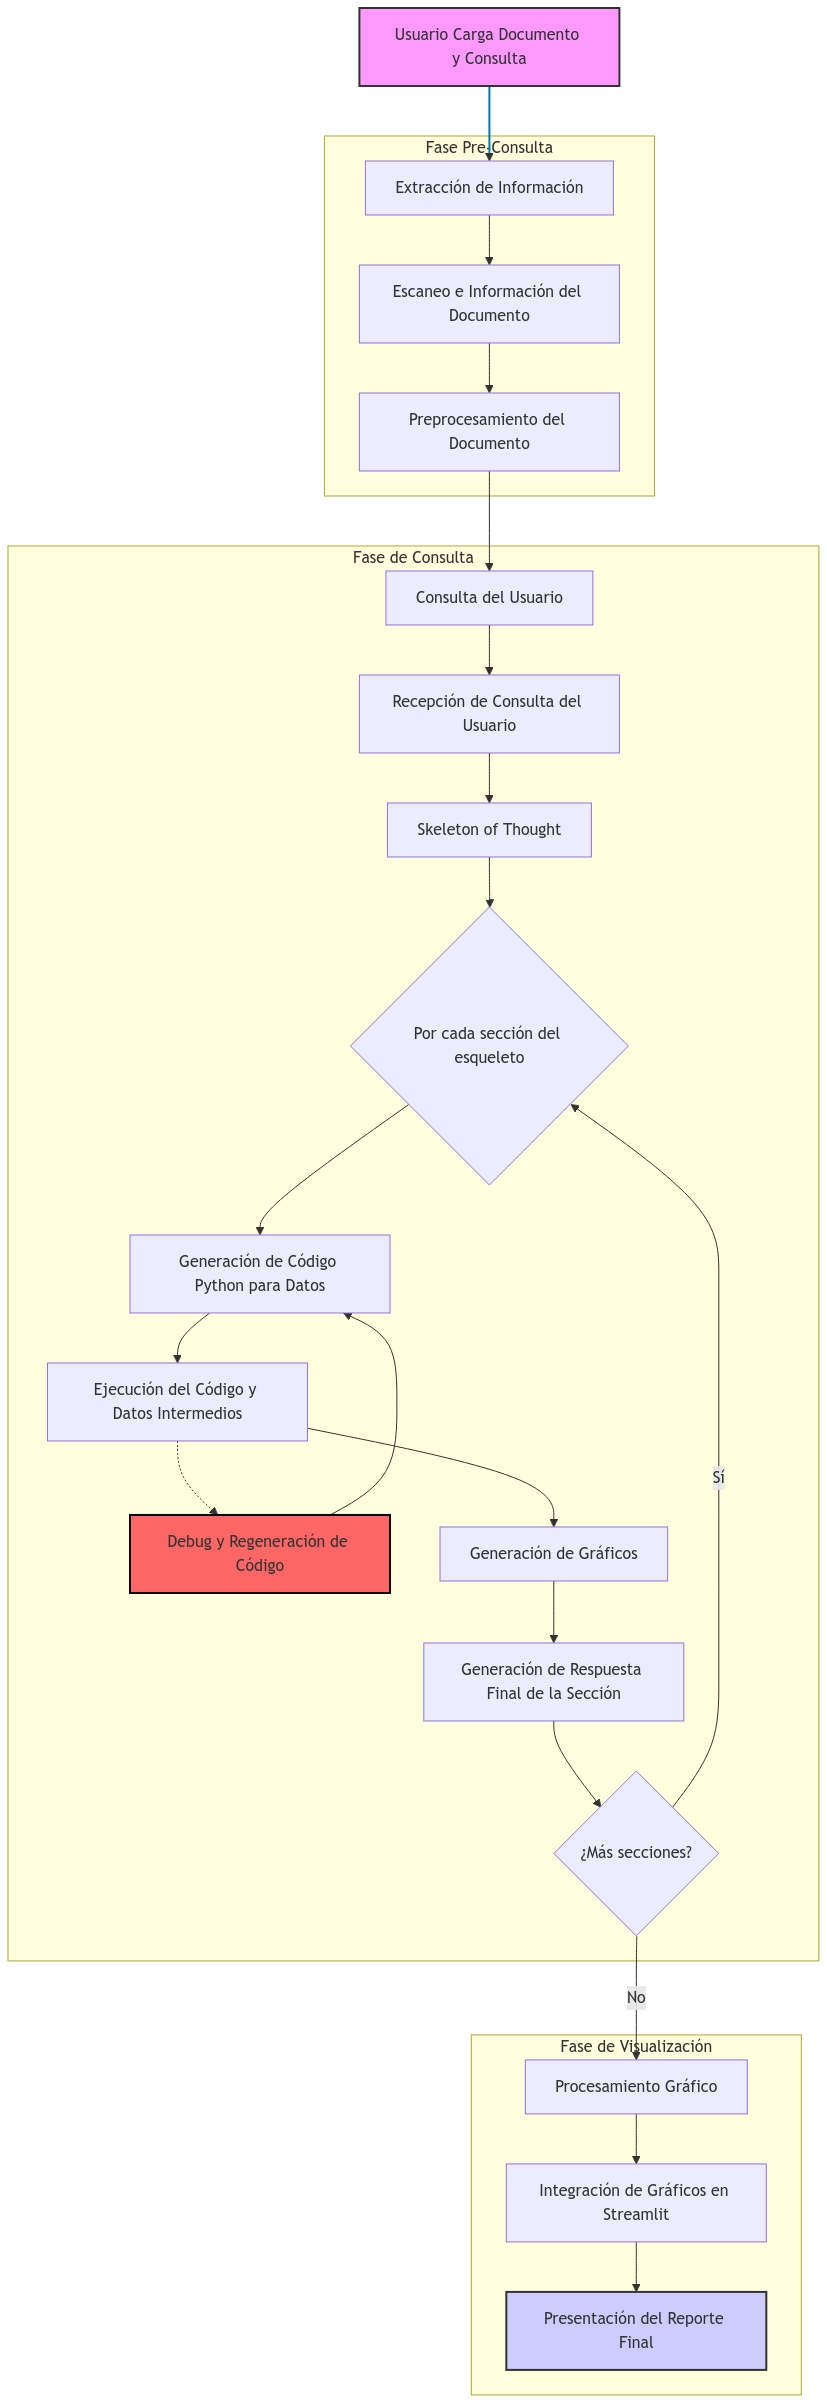
\includegraphics[height=\textheight]{Graphics/graph.png}
	\caption{Flujo de trabajo}
\end{figure}

\subsection{Arquitectura del Sistema y Flujo de Trabajo}

La arquitectura del sistema propuesto se ha diseñado siguiendo un enfoque modular, facilitando la extensibilidad y adaptabilidad a diferentes requerimientos. El flujo de trabajo se divide en etapas claramente definidas, desde la carga del documento por parte del usuario hasta la presentación del reporte final enriquecido con gráficos para una mejor visualizacion de los resultados. Las etapas principales se pueden categorizar en fases previas a la consulta del usuario, procesamiento de la consulta, y generación de la respuesta y visualización.

\subsubsection{Interfaz Gráfica de Usuario (GUI) con Streamlit}

La interfaz gráfica de usuario se ha construido utilizando la librería Streamlit \cite{streamlit}.  Streamlit se seleccionó por su facilidad de uso,  rapidez de desarrollo y la capacidad de crear interfaces web interactivas y de alta calidad con un mínimo de código Python.  Las características de Streamlit aprovechadas en esta implementación incluyen:

\begin{itemize}
	\item \textbf{Componentes interactivos:}  Streamlit proporciona una amplia gama de componentes interactivos (botones, sliders, áreas de texto, selectores de archivos, checkboxes, etc.) que facilitan la creación de interfaces de usuario dinámicas y receptivas.
	\item \textbf{Renderización de código Altair:}  Streamlit integra la capacidad de renderizar gráficos generados con la librería Altair directamente en la interfaz web,  facilitando la visualización de datos.
	\item \textbf{Desarrollo rápido y iterativo:}  Streamlit permite un ciclo de desarrollo rápido e iterativo.  Los cambios en el código Python se reflejan automáticamente en la interfaz web al guardar el archivo,  agilizando la experimentación y el prototipado.
	\item \textbf{Comunidad activa y documentación extensa:}  Streamlit cuenta con una comunidad de usuarios activa y una documentación completa,  lo que facilita la resolución de problemas y el aprendizaje de nuevas funcionalidades.
\end{itemize}
La interfaz web desarrollada con Streamlit proporciona una experiencia de usuario intuitiva y facilita la interacción con el sistema de generación automatizada de reportes.

\subsubsection{Modelos de Lenguaje Utilizados: API de Groq}

La elección del modelo de lenguaje para esta implementación se basó en la premisa de la limitación de recursos computacionales locales para ejecutar modelos de lenguaje de gran escala con un rendimiento adecuado.  En consecuencia,  se optó por utilizar una API gratuita que proporciona acceso gratuito a modelos open-source de alto rendimiento: la API de Groq\cite{groq}.

La API de Groq ofrece acceso a una variedad de modelos open-source punteros,  incluyendo:

\begin{itemize}
	\item \textbf{gemma2-9b-it (Google):}  Modelo de lenguaje desarrollado por Google,  conocido por su eficiencia y buen rendimiento en diversas tareas con un cosumo relativamente bajo de recursos.
	\item \textbf{Familia Llama (Meta):}  Varios modelos de la familia Llama,  desarrollados por Meta (anteriormente Facebook),  incluyendo versiones como Llama 2 y Llama 3.  Se destaca el modelo \textbf{llama-3.3-70b} por sus capacidades demostradas en diversas evaluaciones\cite{llamavsgpt4}.
	\item \textbf{Mixtral-8x7b (Mixtral AI):}  Modelo desarrollado por Mixtral AI,  que ha mostrado un rendimiento competitivo en benchmarks y destaca por su arquitectura Mixture-of-Experts.
\end{itemize}

La utilización de la API de Groq permite experimentar y comparar el rendimiento de diferentes modelos open-source en la tarea de generación de reportes automatizados,  sin requerir una infraestructura computacional local costosa. En futuras investigaciones,  se podría ampliar la experimentación a otros modelos disponibles en la API de Groq o en otras plataformas,  así como explorar estrategias de fine-tuning de los modelos para optimizar su rendimiento en esta tarea específica.


\subsection{Fases Previas a la Consulta del Usuario}

Esta fase inicial se centra en la preparación del entorno y el procesamiento preliminar del documento proporcionado por el usuario. Esta fase consta de los siguientes pasos:

\subsubsection{Carga del Documento por el Usuario}

El sistema inicia con la carga del documento por parte del usuario a través de la interfaz web. Se implementa un componente de carga de archivos el cual forma parte de la librería de streamlit y que admite diversos formatos de documento comunes para el análisis de datos, incluyendo:
\begin{itemize}
	\item \textbf{CSV (.csv):}  Formato de valores separados por comas, ampliamente utilizado para datos tabulares.
	\item \textbf{Excel (.xlsx):}  Formato de hoja de cálculo de Microsoft Excel, capaz de almacenar datos tabulares y fórmulas complejas.
	\item \textbf{Texto (.txt):}  Formato de texto plano, aunque su soporte es más limitado en la implementación actual y se centra en la extracción de información general del documento para contextualizar al LLM.  [Se podría ampliar el soporte para documentos de texto en futuras iteraciones, implementando técnicas de segmentación y análisis semántico más robustas.]
\end{itemize}

La flexibilidad en los formatos de entrada busca maximizar la accesibilidad y usabilidad del sistema para usuarios con diferentes tipos de datos.

\subsubsection{Escaneo e Información del Documento}

Una vez cargado el documento, se procede a un análisis inicial para extraer información relevante que se proporcionará al LLM en etapas posteriores. La función ``get\_document\_info`` se encarga de este proceso, adaptándose al tipo de documento cargado.  Para documentos tabulares (CSV, Excel, JSON), se utiliza la librería Pandas para cargar los datos en un DataFrame, debido a la gran cantidad de funciones que posee esta libreria para un mejor control y analisis de los datos. Esta informacion que se busca extraer del documento en cuestion se busca que sea lo mas corta pero relevante posible ya que debe servir de base para que un LLM tenga una idea del documento en cuestion y como realizar consultas sobre este.

Este enfoque busca emular el comportamiento que seguimos al enfrentarnos a un conjuto de datos que del cual no tenemos infomacion previa. Nosostros como humanos hacemos lo mismo cuando nos enfrentamos a un gran volumne de datos, solo miramos los nombres de las columnas y quizas un par de filas para tener una idea de los tipos de datos con los que estamos trabajando. 

La información extraída incluye:

\begin{itemize}
	\item \textbf{Nombres de las columnas:}  Se obtienen los nombres de las columnas del DataFrame, proporcionando al LLM el vocabulario básico de los datos.
	\item \textbf{Tipos de las columnas:}  Se identifican los tipos de datos de cada columna (numérico, categórico, fecha, etc.),  lo cual es crucial para que el LLM genere código de procesamiento adecuado.
	\item \textbf{Valores Mínimos y Máximos por columna (numéricas):} Se calculan los valores mínimo y máximo para cada columna numérica, ofreciendo al LLM una idea del rango y escala de los datos.
	\item \textbf{Cantidad de Valores Únicos por columna:} Se determina el número de valores únicos en cada columna, lo que puede indicar si una columna es categórica o numérica continua.
	\item \textbf{Valores Faltantes por columna:} Se cuantifica la cantidad de valores faltantes (NaN) en cada columna, información relevante para que el LLM considere estrategias de imputación o manejo de datos faltantes si es necesario.
	\item \textbf{Valores de las primeras filas:} Se muestran las primeras filas del DataFrame tal y como vienen para que el LLM determine correctamente como son los datos de cada columna.
\end{itemize}
Esta información se estructura en un diccionario JSON y se almacenan en una variable ``document\_info`` que se utilizará en las interacciones posteriores con el LLM como parte del prompt.

\subsubsection{Preprocesamiento del Documento}

Para una mejor respuesta estadistica, y datos mas fiables, generalmene se necesita hacer un preprocesamiento de los datos recibidos, ya que estos pueden venir de diferentes fuentes, presentar valores faltantes o algunas inconsistencias en el formato de cada columna. Dicho preprocesamiento puede ser completamente basado en reglas, completamente basado en LLM, o un enfoque hibrido.

El procesamiento basado en reglas especifíca que reglas y criterios tener en cuenta a la hora del preprocesamiento, por ejemplo, las reglas pueden dictar que para cierta fila los datos faltantes se rellenen con el valor de la media de la fila o que ciertos valores outliers necesitan ser topados o normalizados. Este metodo es altamente estructurado y necesita un conocimiento profundo de los datos en cuestion.

El preprocesamiento basado en LLM consiste en utilizar un modelo de lenguaje para rellenar o modificar los datos faltantes asi como categorizar o detectar y corregir incosistencias en los datos. Utilizando el poder del los LLMs permite manejar datos que en principio no esten bien estructurados asi como inferir nuevos datos a partir de texto en lenguaje natural como por ejemplo detectar una valoracion de 1-5 basado en un comentario de un usuario.

El problema que presentan estos tipos de preprocesamiento es que vamos a estar trabajando con un conjuto de datos potencialmente muy grande y del cual no se cuenta con informacion previa, por lo que no podriamos tener reglas predefinidas para las columnas ya que no sabemos que datos se representan en ellas y no podriamos utiliazar las capacidades del LLM para el preprocesado dado el limitado contexto que estos presentan.

Es por esto que se decidió utilizar un enfoque híbrido en cuanto al preprocesado, es decir, utilizar las capacidades de generacion de codigo de los LLM y a partir de estas generar las reglas. Construir un preprocesador de este tipo vendria dado por diseñar un sistema que analize un dataset de entrada,y a partir de este entienda que transformaciones y reglas debe seguir para producir el dataset de salida deseado.

La función ``preprocess\_document`` es la encargada de este proceso, y se divide en dos etapas principales:

\begin{enumerate}
	\item \textbf{Definición de Tareas de Preprocesamiento por el LLM:} Se formula un prompt al LLM solicitándole que analice la información del DataFrame con la informacion del documento que habiamos recolectado anteriormente y sugiera tareas de preprocesamiento relevantes.  El prompt especifica que la respuesta debe ser en formato JSON,  conteniendo una lista de diccionarios, cada uno representando una tarea con detalles como el tipo de tarea, la columna afectada y parámetros adicionales (e.g., formato de fecha).  Las tareas consideradas en el prompt incluyen:
	\begin{itemize}
		\item \textbf{Conversión de Fechas:}  Identificación de columnas que contienen fechas y sugerencia de conversión al tipo `datetime` de Pandas, especificando el formato de fecha si es necesario.
		\item \textbf{Identificación de Columnas Categóricas:}  Reconocimiento de columnas con un número limitado de valores únicos que podrían ser tratadas como variables categóricas.
		\item \textbf{Sugerencias para Columnas No Numéricas No Categóricas:}  Detección de columnas no numéricas que no parecen ser categóricas y sugerencias para su filtrado o tratamiento (e.g., columnas de texto libre que no son relevantes para el análisis numérico).
	\end{itemize}
	
	\item \textbf{Ejecución de Tareas de Preprocesamiento:}  Se itera sobre la lista de tareas de preprocesado que genero el LLM y se genera código Python dinámicamente para cada tarea.  Este código se ejecuta utilizando la función ``execute\_code``, la cual sirve para ejecutar el código en un entorno seguro y controlado, pasando el DataFrame `df`. El comportamiento de esta funcion se detalla mas adelante.
\end{enumerate}

\subsection{Fase de Procesamiento de la Consulta del Usuario}

Una vez que el documento ha sido cargado y preprocesado, el sistema está listo para recibir y procesar las consultas del usuario. Esta fase se compone de los siguientes pasos:

\subsubsection{Recepción de la Consulta del Usuario}

El usuario introduce su consulta en lenguaje natural a través de un área de texto en la interfaz web. Esta consulta representa la pregunta o solicitud de información que el usuario desea obtener a partir del documento cargado.

\subsubsection{Skeleton of Thought: Descomposición del Reporte a Generar}

Se implementa la estrategia ``Skeleton of Thought`` para abordar la complejidad de las consultas.  En lugar de intentar generar una respuesta directa,  se solicita al LLM que a partir de la cosulta del usuario genera la estructura o ``esqueleto`` del reporte a generar, para esto se le provee al modelo los siguientes datos en el ``prompt``.

\begin{itemize}
	\item \textbf{La consulta del usuario en lenguaje natural.}
	\item \textbf{Información relevante sobre el DataFrame (proveniente de ``document\_info``).}
	\item \textbf{Instrucciones claras sobre el formato de respuesta esperado:}  Se indica al LLM que debe responder con un breve análisis de la consulta y una lista de secciones delimitadas dentro de un fragmento de código json. Donde cada seccion se le pide que genere los siguientes datos para un mayor control posterior de la seccion. 
	\begin{itemize}
		\item \texttt{'name'}: - Nombre descriptivo de la sección.
		\item \texttt{'description'}: -  Explicación concisa del propósito de la sección.
		\item \texttt{'data'}: - Descripción del tipo de información que contendrá la sección.  Indicar si se requieren visualizaciones (gráficos, tablas) y sugerir tipos apropiados (ej: "Gráfico de barras para comparar ventas", "Tabla con datos numéricos detallados").
		\item \texttt{'extra\_data'}: -  Sugerencias de información adicional que podría enriquecer la sección y aportar valor al usuario.
	\end{itemize}
\end{itemize}

La respuesta del LLM, que contiene el análisis y la lista de secciones,  se almacena como ``skeleton\_response`` y se muestra en la interfaz web para la revisión del usuario en caso de tener activado el modo depuracion, del cual hablaremos mas adelante.

\subsubsection{Generación de Código Python para obtener datos consisos}

Para cada seccion identificada en el paso anterior, se solicita al LLM que genere código Python utilizando la librería Pandas para operar sobre el DataFrame $`df`$.  El proceso se repite para cada tarea seccion individualmente.  El prompt formulado al LLM en este paso incluye:

\begin{itemize}
	\item \textbf{El nombre, la descripcion, y los datos generados en el proceso de creacion del esqueleto del reporte.}
	\item \textbf{Información relevante sobre el DataFrame:} proveniente de la variable  ``document\_info``.
	\item \textbf{Instrucciones sobre el formato de respuesta esperado:} Se especifica que el LLM debe responder con código Python encapsulado entre delimitadores.
\end{itemize}
Ademas se utiliza una tecnica llamada ``constraint prompting`` en donde se le restringe las capacidades generativas del LLM a seguir una serie de reglas, en este caso se le pide que el codigo python a generar no puede modificar el dataframe original, que los datos relevantes que desee recuperar los debe almacenar en una variable local llamada ``response``, y que no recupere grandes volumenes de datos, solo la informacion relevante que sea capaz de extraer usando codigo python de estos.

La respuesta del LLM, que contiene el código Python se parsea para determinar solamente la region donde se encuentra el codigo, se almacena como ``code\_response`` y se muestra en la interfaz web en caso de depuracion.

\subsubsection{Ejecución del Código y Obtención de Resultados Intermedios}

El código Python generado para cada tarea atómica se ejecuta utilizando nuevamente la función ``execute\_code``.  Esta función ejecuta el código en un entorno seguro,  pasando el DataFrame $`df$` como variable local.  El resultado de la ejecución como se le habia pedido al modelo se deben encontrar en la variable local response. Si la ejecución es exitosa,  los resultados (que pueden ser DataFrames, series, valores numéricos, diccionarios, etc.).  Si ocurre un error durante la ejecución,  se captura el error y se muestra en la interfaz web en caso de depuracion y  luego se intenta utilizar nuevamente el LLM para corregir el codigo python en cuestion.

La funcion ``execute\_code`` contiene un parametro opcional ``max\_retries``, el cual se utiliza para evitar caer en un ciclo infinito donde no se pueda corregir el codigo en cuestion. Para intentar arreglar el codigo se acude nuevamente al modelo del lenguaje, este proceso se realiza mediante la funcion ``debug\_and\_regenerate\_code``, la cual recibe como parametros el codigo que se ejecuto y dio error y el mensaje de error lanzado, y a partir de esos datos se le pide al LLM que genere un nuevo codigo python, el cual automaticamete se parsea y se vuelve a intentar ejecutar.

\subsubsection{Generación de Graficos}

Para mejorar la visualizacion de los datos y la calidad de los reportes se hace necesario la inclusion de elementos graficos que permitan al usuario ver y entender una mayor cantidad de datos y su comportamiento. Para la generacion de estos graficos seguimos la misma idea de el punto anterior de obtencion de datos, como no pudemos proveer a los LLM con todo el conjunto de datos para que este renderize una grafica o tabla a partir de esto, lo que hacemos es pedirle que genere codigo python que sea capaz de generar estos graficos.

Para este proposito utilizamos la libreria altair\cite{altair}, una libreria capaz de generar varios tipos de graficos a partir de un dataframe en pandas, estas facilidades unidos a la funcionalidad de streamlit de renderizar dichos graficos directamente en la web con una sola intruccion, hacen de esta libreria una opcion ideal para este trabajo.

En este paso se siguen las mismas ideas, en cuanto a la estructura del prompt, que las vistas en la seccion \textbf{Generación de Código Python para obtener datos consisos}. Con la diferencia que se le hace saber al modelo que la libreria altair ya esta importada como ``alt``, y que las respuestas deben ser una lista de diccionarios que contengan la siguiente informacion:

\begin{itemize}
	\item \textbf{name} :- Nombre del grafico, este se utiliza luego como un id para acceder al grafico en cuestion.
	\item \textbf{description} :- Una breve descripcion del grafico en cuestion y los datos que representa para que a la hora de generar la respuesta final a partir de esta informacion el modelo de lenguaje sepa en que posicion ubicarlo.
	\item \textbf{c} :- Referencia al objeto Altair del grafico.
\end{itemize}

\subsubsection{Generación de la Respuesta Final de la seccion}

Para la generación de la sección final del reporte, se recurre al LLM, al cual se le proporciona toda la información procesada y relevante para la sección en cuestión. Esto incluye los datos extraídos y calculados previamente, la información contextual del documento analizado, y las descripciones de las visualizaciones gráficas generadas. Con el objetivo de facilitar la integración de gráficos dentro del flujo textual del reporte, se instruye al LLM para que utilice una sintaxis inspirada en markdown. Específicamente, se le indica que inserte un bloque de código ```chart <nombre\_del\_gráfico> ``` en aquellos puntos donde considere pertinente incluir una visualización.

Una vez obtenida la respuesta del LLM, se procede a analizarla (parsearla) para identificar estos marcadores de gráficos. Posteriormente, estos marcadores son reemplazados programáticamente por las correspondientes gráficas generadas con Altair, permitiendo una integración fluida y dinámica de texto y visualizaciones en la sección del reporte final presentada en Streamlit.


\chapter{Validación de la Implementación y Experimentos}\label{chapter:implementation}

En este capítulo, se detalla la implementación de la solución propuesta, analizando un caso de prueba detalladamente paso a paso.  En cada etapa de este caso de prueba, se describe el proceso seguido al detalle. Para este caso de prueba estaremos usando el modelo Llama3.3-70b, la elección del modelo Llama3.3-70b se justifica por su rendimiento superior en cuanto a tiempo de respuesta, según lo evidenciado en pruebas preliminares.

En este caso de prueba, estaremos utilizando el dataset \href{https://huggingface.co/datasets/sayanroy058/Business-Sales/viewer}{\textbf{Business-Sales}}, que comprende datos de transacciones de ventas de automóviles. Este dataset resulta ideal para evaluar la capacidad del modelo Llama3.3-70b, tanto en la generación de informes automáticos como en la resolución de consultas en lenguaje natural debido a las siguientes consideraciones.

\subsubsection{Consideraciones sobre el Dataset}
Antes de describir las características principales del dataset, es fundamental destacar algunos aspectos críticos que influyen en su procesamiento y análisis.
\begin{itemize}
	\item{Datos Faltantes:}
	Existen valores faltantes en algunas columnas, lo que requiere que el LLM analice e implemente alguna técnica de imputación para completar estos valores.
	
	\item{Columnas Irrelevantes:}
	Algunas columnas, como VIN (Número de Indentificación del Vehículo), contienen información única para cada vehículo y no aportan valor para los análisis o reportes generales. Por lo tanto, el modelo debería identificar esta irrelevancia y, ya sea desecharla en el preprocesamiento o, al menos, no utilizarla al generar información.
	
	\item{Columnas con Abreviaturas:}
	Existen columnas como MMR (Manheim Market Report) cuyo significado no es explícito. El modelo deberá razonar en contexto para comprender su relevancia y cómo utilizarla en el análisis.
	
	\item{Interpretación de Rangos:}
	Algunas columnas, como \textit{condition}, presentan valores numéricos cuya interpretación no es inmediata. El modelo deberá inferir el rango y significado de estos valores para obtener resultados adecuados.
	
	\item{Razonamiento sobre Datos Heterogéneos:}
	Las columnas combinan datos categóricos, numéricos y textuales, lo que pone a prueba la capacidad del modelo para generalizar y extraer patrones útiles.
	
	\item{Gran cantidad de datos:}
	El dataset cuenta con cerca de 600 mil entradas, lo cual hace que sea imposible pasarlo completamente como contexto a ninguno de los modelos de lenguaje actuales.
\end{itemize}

\section{Interfaz}
Al acceder al sitio web proporcionado por Streamlit al ejecutar el programa, se presenta una página web que consta de dos columnas principales: una columna central más espaciosa, que constituye el contenido principal de la página, y una columna lateral a la izquierda, destinada a la configuración.

\subsection{Columna de configuracion}
La columna de configuración es una columna lateral estrecha que permite configurar el modelo de lenguaje a utilizar de entre los disponibles en la API de Groq.  Adicionalmente, incluye un control deslizante (slider) para seleccionar la cantidad máxima de tokens a generar por el modelo. Esto proporciona un mayor control sobre las invocaciones a la API y ayuda a mantenerse dentro de los límites establecidos por el sitio web.

Esta columna también incluye una casilla de verificación (checkbox) deshabilitada por defecto, denominada "Debug". Al activarla, se habilita una nueva columna a la derecha de la columna principal que muestra el contenido detallado de cada paso del proceso. En esta columna se visualizan las llamadas y respuestas del LLM, los resultados de la ejecución del código generado, el proceso de preprocesamiento con el detalle de cada tarea identificada, y prácticamente todo lo que ocurre durante la generación del reporte.

\subsection{Culumna Principal}
La columna principal presenta un encabezado con el título \textbf{Generador de Reportes Automatizados con LLM} y, debajo, un componente para la carga de archivos.  Este componente permite la carga de archivos tanto mediante la interfaz de carga de archivos propia del sistema operativo, como mediante la funcionalidad de arrastrar y soltar. Una vez que se carga el archivo comienza el proceso de extraer los datos relevantes del mismo.

A partir de los datos extraídos, se solicita al LLM que genere una lista de tareas de preprocesamiento.  Estas tareas pueden variar desde operaciones predefinidas, como marcar una columna como categórica o convertir una columna de fechas a objetos de fecha de Python, hasta tareas más complejas para las cuales se le solicita que proporcione el código Pandas correspondiente. En el caso que se analiza, la lista de tareas generada por el modelo fue la siguiente:


\definecolor{jsoncolor}{rgb}{0.12,0.55,0.82}

\begin{lstlisting}
		{"tarea": "convertir_fecha", "columna": "saledate"}, 
		{"tarea": "identificar_categorica", "columna": "make"}, 
		{"tarea": "identificar_categorica", "columna": "model"}, 
		{"tarea": "identificar_categorica", "columna": "trim"}, 
		{"tarea": "identificar_categorica", "columna": "body"}, 
		{"tarea": "identificar_categorica", "columna": "transmission"}, 
		{"tarea": "identificar_categorica", "columna": "state"}, 
		{"tarea": "identificar_categorica", "columna": "condition"}, 
		{"tarea": "identificar_categorica", "columna": "color"}, 
		{"tarea": "identificar_categorica", "columna": "interior"}, 
		{"tarea": "identificar_categorica", "columna": "seller"}, 
		{"tarea": "filtrar", "columna": "vin", "sugerencia": "Eliminar columna, no se utiliza para el analisis"}, 
		{"tarea": "filtrar", "columna": "odometer", "sugerencia": "Filtrar valores outliers"}, 
		{"tarea": "filtrar", "columna": "condition", "sugerencia": "Filtrar valores outliers"}, 
		{"tarea": "filtrar", "columna": "mmr", "sugerencia": "Eliminar filas con datos faltantes"}, 
		{"tarea": "filtrar", "columna": "sellingprice", "sugerencia": "Eliminar filas con datos faltantes"}, 
		{"tarea": "pandas", "codigo": "df = df[df.condition < 50] # Filtrar condicion extrema"}, 
		{"tarea": "pandas", "codigo": "df = df[df.odometer < 50000] # Filtrar kilometraje extremo"}, 
		{"tarea": "pandas", "codigo": "df = df[df.mmr > 0] # Filtrar valores negativos de MMR"}, 
		{"tarea": "pandas", "codigo": "df = df[df.sellingprice > 0] # Filtrar valores negativos de precio de venta"} ]
\end{lstlisting}

Como se puede observar, el modelo generó un JSON con un arreglo de tareas de preprocesamiento a realizar.  Entre estas tareas, se destaca la eliminación de la columna \textit{vin}, la eliminación de valores negativos en la columna \textit{sellingprice}, y la eliminación de valores extremos en la columna \textit{condition}.  Esto demuestra que el proceso de extracción de información previo fue exitoso, ya que el modelo logró inferir las columnas relevantes, el rango de valores esperado en cada una, y los posibles valores atípicos o ``ruido`` en el dataset.

Una vez finalizado el preprocesamiento, se notifica al usuario el resultado, indicando si fue satisfactorio o si ocurrió algún error. En cualquier caso, debajo de estas notificaciones aparece un cuadro de texto donde se solicita al usuario que introduzca una consulta. La consulta debe ser en lenguaje natural y relacionada con el documento cargado. Adicionalmente, se sugieren al usuario tres posibles consultas relevantes al documento subido.

Para evaluar las capacidades del LLM, se le solicita generar un reporte de ventas de la marca Kia en el año 2014. Esta consulta permitirá verificar si el modelo es capaz de filtrar los datos necesarios para elaborar la respuesta, así como su habilidad para generar gráficos relevantes que complementen la información. 

\section{Generando el reporte}
Tras cargar el documento y completar el preprocesamiento, se introduce la siguiente consulta:

\textit{¿Cómo se comportaron las ventas de Kia en 2014 en relación con las del año anterior?}

Como primer paso, el modelo genera el \textbf{esqueleto del reporte}. Para cada sección del esqueleto, el modelo proporciona el nombre de la sección, una descripción, y sugerencias sobre cómo estructurar los gráficos o qué datos deben mostrar.

En este caso el modelo nos proporcionó el siguiente esqueleto:

\noindent\colorbox{gray!5}{ % Fondo gris muy claro
	\noindent\fbox{ % Cuadro
		\begin{minipage}{\dimexpr\linewidth-2\fboxsep-2\fboxrule\relax}
			\begin{description}
				\item[\textbf{Sección Introducción}]
				\begin{itemize}
					\item \textbf{Descripción:} Breve contexto del análisis de las ventas de Kia en 2014 y comparación con 2013
				\end{itemize}
				\item[\textbf{Sección Ventas de Kia en 2014}]
				\begin{itemize}
					\item \textbf{Descripción:} Presentación detallada de las ventas de Kia en 2014
				\end{itemize}
				\item[\textbf{Sección Ventas de Kia en 2013}]
				\begin{itemize}
					\item \textbf{Descripción:} Presentación detallada de las ventas de Kia en 2013
				\end{itemize}
				\item[\textbf{Sección Comparación de Ventas entre 2013 y 2014}]
				\begin{itemize}
					\item \textbf{Descripción:} Comparación de las ventas de Kia en 2013 y 2014
				\end{itemize}
				\item[\textbf{Sección Análisis de la Tendencia de las Ventas}]
				\begin{itemize}
					\item \textbf{Descripción:} Análisis de la tendencia de las ventas de Kia en 2014 en comparación con 2013
				\end{itemize}
				\item[\textbf{Sección Conclusiones y Recomendaciones}]
				\begin{itemize}
					\item \textbf{Descripción:} Resumen de los hallazgos y conclusiones del análisis de las ventas de Kia en 2014
				\end{itemize}
			\end{description}
		\end{minipage}
}}

A partir de este esqueleto, se inicia la generación del reporte sección por sección. El primer paso para crear cada sección, como se planteó en el capítulo anterior, es obtener datos del dataframe mediante código Python generado por el LLM. En esta ocasión, el modelo generó el siguiente código: 


\begin{lstlisting}
	import pandas as pd
	
	# Suponemos que el dataframe 'df' ya esta cargado
	
	# Calculamos el numero de ventas de Kia en 2014 y 2013
	ventas_2014 = len(df[(df['year'] == 2014) & (df['make'] == 'Kia')])
	ventas_2013 = len(df[(df['year'] == 2013) & (df['make'] == 'Kia')])
	
	# Calculamos el porcentaje de aumento o disminucion de ventas
	if ventas_2013 != 0:
	porcentaje_cambio = ((ventas_2014 - ventas_2013) / ventas_2013) * 100
	else:
	porcentaje_cambio = 0
	
	# Creamos un diccionario con la informacion necesaria para la seccion de introduccion
	response = {
		'ventas_2014': ventas_2014,
		'ventas_2013': ventas_2013,
		'porcentaje_cambio': porcentaje_cambio,
		'relevancia': 'El analisis de las ventas de Kia en 2014 y 2013 es relevante para entender el comportamiento del mercado y la estrategia de la empresa en ese periodo.'
	}
	
	print(response)
\end{lstlisting}

Nótese que el modelo identifica correctamente el objetivo y los datos necesarios para la introducción.  En este caso, decide obtener el número total de ventas de ambos años y el porcentaje de cambio interanual. El modelo también incluye, aunque con una ligera imprecisión, una cadena de texto de "relevancia".Esta cadena parece ser una anotación para la generación del reporte, donde se subraya la relevancia del análisis de ventas de estos años para comprender el comportamiento del mercado.

El segundo paso para la generación de cada sección era identificar y generar gráficos que pudieran facilitar el análisis de los datos recopilados por parte del usuario. En esta ocasión, tras generar inicialmente un código erróneo, el modelo logró producir los siguientes gráficos.

\begin{figure}[H] % Usamos h! para forzar la posición aquí si es necesario, pero considera htbp para más flexibilidad
	\centering % Centrar todo el conjunto de figuras horizontalmente
	\begin{minipage}{0.48\textwidth} % Ajusta el ancho según necesites (ej. 0.48 para dejar espacio entre figuras)
		\centering
		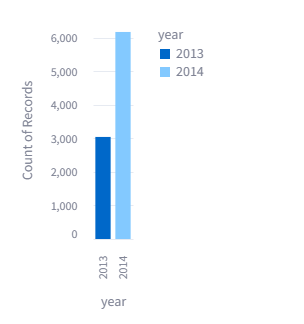
\includegraphics[height=150px]{grafica_anual.png} % Reemplaza con tu archivo real
		\caption{Número total de ventas de Kia por año}
		\label{fig:ejemplo_introduccion_grafico_anual}
	\end{minipage}
	\begin{minipage}{0.48\textwidth} % Ajusta el ancho según necesites
		\centering
		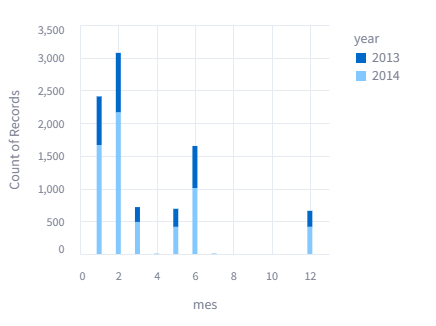
\includegraphics[height=150px]{grafica_mensual.png} % Reemplaza con tu archivo real
		\caption{Distribución de ventas de Kia por mes}
		\label{fig:ejemplo_introduccion_grafico_mensual}
	\end{minipage}
\end{figure}

Error detectado en la primera ejecución del código generado:
\textbf{\textit{Error message: Tz-aware datetime.datetime cannot be converted to datetime64 unless utc=True, at position 127}}

Posteriormente, al solicitar al modelo que genere la sección del reporte utilizando los datos obtenidos y estos gráficos, se muestra la primera sección del reporte en la columna principal. A partir de aquí, el resto de las secciones se generan de forma similar.

\begin{figure}[H] % Usamos h! para forzar la posición aquí si es necesario, pero considera htbp para más flexibilidad
	\centering % Centrar todo el conjunto de figuras horizontalmente
	\begin{minipage}{0.48\textwidth} % Ajusta el ancho según necesites (ej. 0.48 para dejar espacio entre figuras)
		\centering
		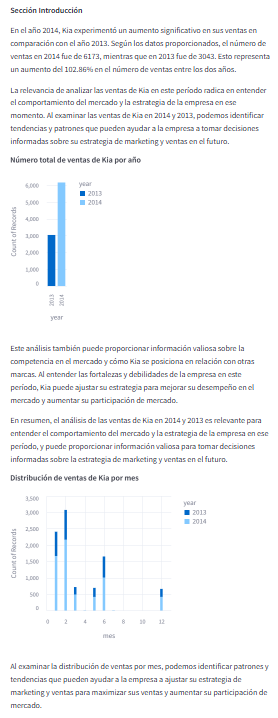
\includegraphics[height=\textheight]{intro.png} % Reemplaza con tu archivo real
		\caption{Sección Introducción}
		\label{fig:ejemplo_introduccion}
	\end{minipage}
\end{figure}




\subsection{Experimentos y Líneas de Investigación}

La implementación descrita sienta las bases para una serie de experimentos y líneas de investigación que podrían explorar y mejorar las capacidades del sistema.  Algunas áreas de interés incluyen:

\begin{itemize}
	\item \textbf{Evaluación comparativa de modelos LLM:}  Realizar una evaluación sistemática comparando el rendimiento de diferentes modelos LLM disponibles en la API de Groq (y otras plataformas) en la tarea de generación de reportes automatizados.  Métricas a considerar podrían incluir la precisión del código generado,  la relevancia y coherencia de las respuestas,  la velocidad de respuesta,  y la calidad de las visualizaciones.
	\item \textbf{Optimización de prompts y estrategias de prompt engineering:}  Experimentar con diferentes prompts y técnicas de prompt engineering (e.g., few-shot learning, chain-of-thought prompting, constraint prompting) para mejorar la calidad de las respuestas,  la precisión del código generado y el control sobre el estilo y el tono del reporte.
	\item \textbf{Desarrollo de mecanismos de validación y corrección de código:}  Implementar mecanismos para validar el código Python generado por el LLM antes de su ejecución,  y para permitir la corrección manual o automática del código en caso de errores.  Esto podría incluir pruebas unitarias generadas por el LLM o la integración de un intérprete de Python en el bucle de retroalimentación.
	\item \textbf{Expansión de las capacidades de preprocesamiento:}  Ampliar el rango de tareas de preprocesamiento que el sistema puede realizar automáticamente,  incluyendo tareas más complejas como la imputación de valores faltantes,  la normalización de datos,  la detección de outliers,  y la ingeniería de características.
	\item \textbf{Mejora de la generación de visualizaciones:}  Desarrollar un sistema más inteligente y flexible para la generación de visualizaciones,  que seleccione automáticamente el tipo de gráfico adecuado,  permita la personalización por parte del usuario,  y genere tablas formateadas cuando sea apropiado.  Integrar el LLM para que sugiera visualizaciones relevantes y genere descripciones textuales de las mismas.
	\item \textbf{Soporte para bases de datos y fuentes de datos externas:}  Extender el sistema para que pueda interactuar directamente con bases de datos y otras fuentes de datos externas,  en lugar de limitarse a documentos cargados por el usuario.  Esto requeriría la implementación de mecanismos para la conexión a bases de datos,  la generación de consultas SQL u otros lenguajes de consulta,  y la integración de los resultados en el flujo de trabajo de generación de reportes.
	\item \textbf{Evaluación con usuarios reales y estudios de caso:}  Realizar estudios de caso y evaluaciones con usuarios reales para medir la usabilidad,  utilidad y efectividad del sistema en escenarios prácticos.  Recopilar feedback de los usuarios para identificar áreas de mejora y refinar el diseño del sistema.
\end{itemize}

Estas líneas de investigación representan direcciones prometedoras para avanzar en el desarrollo de sistemas de generación automatizada de reportes más potentes,  flexibles y adaptables a las necesidades de los usuarios.

\backmatter

\begin{conclusions}
    La presente tesis ha demostrado la viabilidad y el potencial de la automatización de la generación de reportes mediante la integración de LLMs y bases de conocimiento estructuradas. A través del desarrollo e implementación de un sistema funcional, se han alcanzado las siguientes conclusiones principales:
    \begin{itemize}
    \item{Efectividad del Enfoque Skeleton-of-Thought:} La estrategia de decodificación Skeleton-of-Thought ha demostrado ser efectiva para guiar a los LLMs en la generación de reportes estructurados y coherentes. La descomposición del proceso en la creación de un esqueleto y la posterior expansión detallada ha mejorado la organización y la calidad del contenido generado. Este enfoque permite además generar reportes más largos y detallados que los que pudieran ser generados solamente por una consulta a un LLM.
    
    \item{Potencial del Prompt Engineering:} Las técnicas de prompt engineering han sido cruciales para dirigir el comportamiento del LLM, controlando el estilo, el tono y la precisión de la información en los reportes generados. La experimentación con diferentes tipos de prompts ha revelado la importancia de un diseño cuidadoso para obtener resultados óptimos. La técnica de ``constrain prompting`` ha facilitado que incluso modelos pequeños sigan correctamente la estructura de respuestas propuestas en el prompt
    
	\item{Generación de Código y Gráficos Automatizada:}  El sistema destaca por su capacidad de generar automáticamente código Python para la extracción y el preprocesamiento de datos, así como para la creación de visualizaciones gráficas relevantes. Esta automatización es crucial para la eficiencia y escalabilidad del sistema. Aunque inicialmente se observaron errores en el código generado, la implementación de un mecanismo de retroalimentación permitió que el modelo, tras recibir la notificación del error específico, pudiera corregirlo en la mayoría de los casos, requiriendo generalmente solo un intento para lograr una ejecución exitosa.
    
    \item{Limitaciones y Desafíos:} A pesar de los avances, se reconocen limitaciones inherentes a los LLMs, como la posible generación de información incorrecta o alucinaciones, aun cuando le damos los datos correctos recibidos mediante codigo python.
\end{itemize}
    En resumen, esta tesis ha proporcionado una base sólida para la automatización de la generación de reportes, demostrando que la combinación de LLMs, bases de conocimiento y técnicas de prompt engineering ofrece una vía prometedora para mejorar la eficiencia y la accesibilidad en el manejo de información.
    
\end{conclusions}

\begin{recomendations}
    A partir de las conclusiones de esta tesis, se proponen las siguientes recomendaciones para futuras investigaciones y desarrollos:
    
    Se recomienda realizar una evaluación sistemática y comparativa de diversos modelos LLM, tanto open-source como propietarios, en la tarea específica de generación de reportes. Esta evaluación debería considerar métricas cuantitativas (precisión, coherencia, completitud) y cualitativas (utilidad, claridad, relevancia). Asi como la posibilidad de utilizar fine-tunning para tener un modelo mas robusto en la generación de reportes.
    
    Una posible mejora que se plantea en casi todos los programas que  utilizan skeleton-of-thougt como estructura principal es la de paralelización, es decir, ir generando cada seccion en un hilo o proceso de trabajo distinto lo que permitiria reducir el tiempo de generacion de los reportes. En este trabajo no se abarco esa posibilidad debido a las limitaciones de la API.
    
    Es fundamental continuar investigando y desarrollando técnicas de prompt engineering más avanzadas y sofisticadas. Se sugiere explorar estrategias como el aprendizaje few-shot más elaborado y el chain-of-thought prompting para razonamiento más complejo.

    Un paso evolutivo importante sería extender el sistema para que pueda interactuar directamente con bases de datos relacionales, NoSQL, APIs y otras fuentes de datos externas. Esto requeriría desarrollar mecanismos para la conexión segura a estas fuentes, la generación de consultas en diferentes lenguajes (SQL, GraphQL, etc.) y la integración fluida de los resultados en el proceso de generación de reportes.
    
    Se recomienda realizar estudios de caso en dominios específicos (finanzas, medicina, ingeniería, etc.) para evaluar la efectividad del sistema en escenarios prácticos y relevantes. Es crucial llevar a cabo evaluaciones con usuarios reales (analistas de datos, profesionales de negocios, etc.) para medir la usabilidad, utilidad y el impacto del sistema en entornos de trabajo reales. Recopilar feedback de los usuarios sería esencial para identificar áreas de mejora y refinar el diseño del sistema para satisfacer las necesidades reales.
    
    Dado el potencial de los LLMs para generar contenido sesgado o incorrecto, se recomienda investigar activamente estrategias para mitigar estos problemas en el contexto de la generación de reportes. Esto podría incluir técnicas de fact-checking automatizado, el uso de bases de conocimiento verificadas, y el desarrollo de prompts que fomenten la objetividad y la precisión.
    
    Implementar estas recomendaciones permitiría avanzar significativamente en el desarrollo de sistemas de generación automatizada de reportes más potentes, confiables y adaptados a las necesidades de diversos usuarios y dominios.
\end{recomendations}

\printbibliography

\end{document}